\documentclass{article}
\usepackage[x11names, rgb]{xcolor}
\usepackage[utf8]{inputenc}
\usepackage{tikz}
\usetikzlibrary{snakes,arrows,shapes}
\usepackage{amsmath}
%
%

%

%

\begin{document}
\pagestyle{empty}
%
%
%

\enlargethispage{100cm}
% Start of code
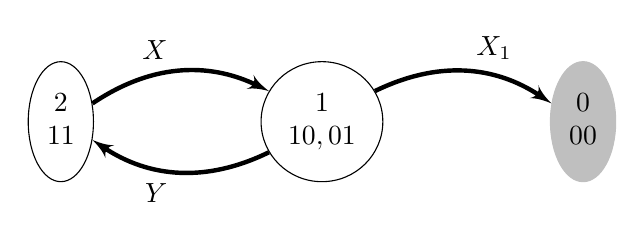
\begin{tikzpicture}[>=latex',line join=bevel,]
%%
\node (1) at (121bp,20.797bp) [draw,ellipse] {$\begin{matrix}1 \\ 10,01 \end{matrix}$};
  \node (0) at (215bp,20.797bp) [draw=lightgray,fill=lightgray,ellipse] {$\begin{matrix}0 \\ 00 \end{matrix}$};
  \node (2) at (27bp,20.797bp) [draw,ellipse] {$\begin{matrix}2 \\ 11 \end{matrix}$};
  \draw [->,ultra thick] (1) to[bend left] node[auto] {$X_1$} (0);
  \draw [->,ultra thick] (2) to[bend left] node[auto] {$X$} (1);
  \draw [->,ultra thick] (1) to[bend left] node[auto] {$Y$} (2);
  %\draw [->,ultra thick] (0) to[bend left] node[auto] {$Y$} (1);
%
\end{tikzpicture}
% End of code

%
\end{document}
%



